\documentclass[12pt]{article}
\usepackage{sbc-template}
\usepackage{graphicx,url}
\usepackage[utf8]{inputenc}
\usepackage[brazil]{babel}
\usepackage{color}
\usepackage{listings}

%%%%%%%%%%%%%%%%%%%%%%%%%%%%%%%%%%%%%%%%%%%%%%%%%%%%
% C O N F I G U R A Ç Õ E S  D O S   C Ó D I G O S %
%%%%%%%%%%%%%%%%%%%%%%%%%%%%%%%%%%%%%%%%%%%%%%%%%%%%

\lstset{
	numbers=left,
	stepnumber=1,
	firstnumber=1,
	numberstyle=\scriptsize,
	extendedchars=true,
	breaklines=true,
	frame=single,
	showstringspaces=false,
  aboveskip=1.5em,
	xleftmargin=2.5em,
	framexleftmargin=2em,
	basicstyle=\scriptsize,
}

\renewcommand{\lstlistingname}{Código}
\renewcommand{\lstlistlistingname}{Lista de Códigos}

\sloppy

\title{Aprendizagem de Máquina (2020/Período Especial) - Redes Neurais}

\author{Diogo C. T. Batista\inst{1}}

\address{Universidade Federal do Paraná (UFPR)\\
	Curitiba -- Paraná -- Brasil
	\email{diogo@diogocezar.com}
	}

\begin{document}

\maketitle

\section{Introdução}

Neste laboratório, foi considerada uma base de dados com os meses do ano. As imagens são representações manuscritas das palavras que compreendem os meses: Janeiro, Fevereiro, Março, Abril, Maio, Junho, Julho, Agosto, Setembro, Outubro, Novembro e Dezembro. Por tanto, temos 12 classes. A Figura \ref{fig:image_months} demostra alguns exemplos dessas imagens.

\begin{figure}[!htb]
  \centering
  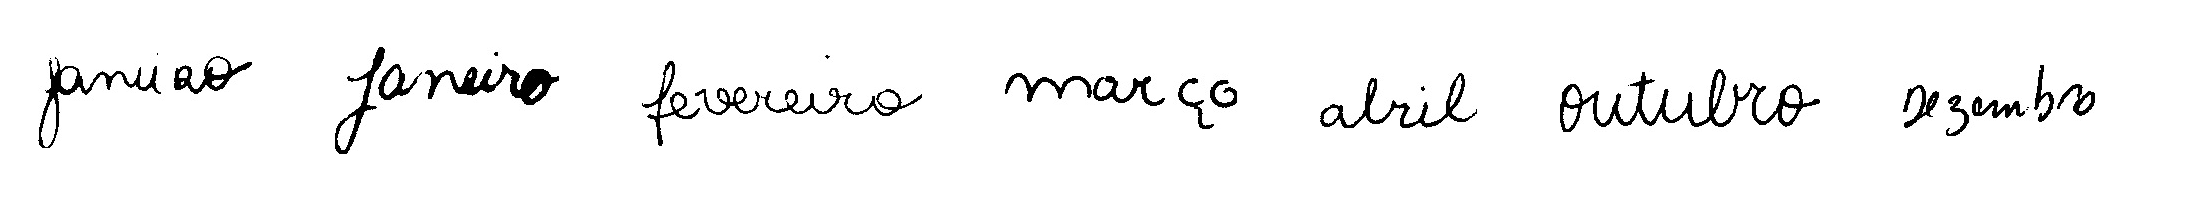
\includegraphics[width=35em]{images/image_months.png}
  \caption{Exemplos dos meses manuscritos}
  \label{fig:image_months}
\end{figure}

As implementações para este laboratório foram relaizadas na plataforma Google Colab. Foram realizadas as seguintes etapas: Preparações, Definição dos Modelos, Execução do Modelo LeNet5 sem Data Augmentation, Execução de um Modelo Personalizado sem Data Augmentation, Implementação de Data Augmentation, Execução do Modelo LeNet5 com Data Augmentation, Execução de um Modelo Personalizado com Data Augmentation, Extração de Características e Implementação do SVM com as Características Extraídas.

Na sequência cada uma das etapas será detalhada, seguido da análise dos resultados obtidos em cada uma das etapas, bem como as suas comparações.

Para a execução dos experimentos, utilizou-se os Frameworks Keras e Sklearn.

\section{Preparações}

Nesta etapa do laboratório foram realizadas as preparações para os experimentos: Habilitação da GPU, Importação dos dados hospedados no GitHub, Definição dos Arquivos de Entrada e Definição das Funções Auxiliares.

Com a execução dos experimentos foi realizad no Google Colab, os experimentos foram realizados com a habilitação do processamento via GPU.

Na definição das funções auxiliares, a ideia foi definir possíveis componentes reutilizáveis nos experimentos, encapsulando implementações em funções reutilizáveis.

\section{Definição dos Modelos}

Definiu-se também os modelos como funções. O primeiro modelo utilizado foi o LeNet 5, suas camadas estão representadas na Figura \ref{fig:image_lenet}

\begin{figure}[!htb]
  \centering
  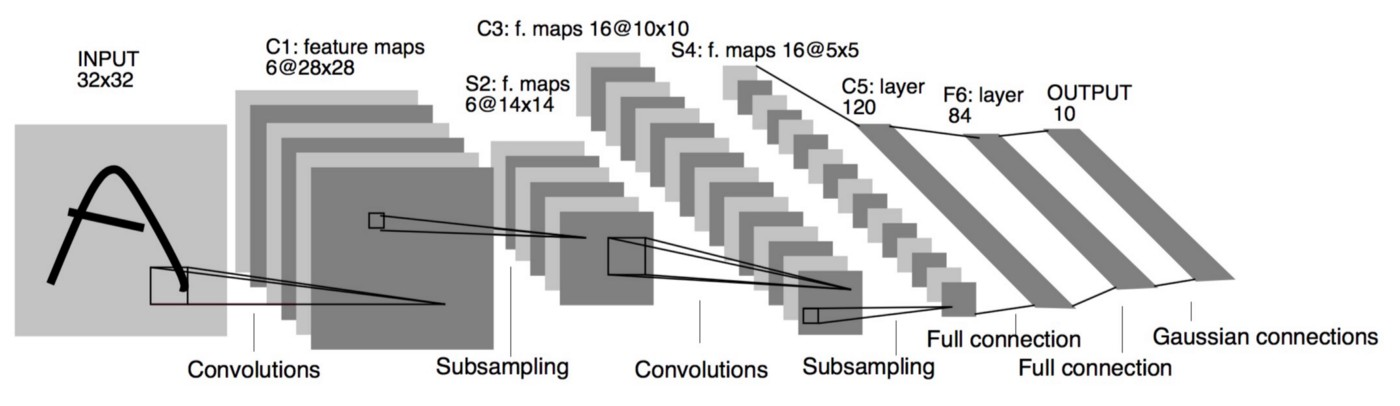
\includegraphics[width=35em]{images/image_lenet.jpeg}
  \caption{Exemplos das camadas utilizadas pelo modelo LeNet5}
  \label{fig:image_lenet}
\end{figure}

O segundo modelo, é o mesmo utilizado nas demonstrações em aula e  implementa as seguintes as camadas detalhadas no Código \ref{code:modelo_personalizado}.

\begin{lstlisting}[caption={Modelo Personalizado},captionpos=b,frame=single,label={code:modelo_personalizado}]
model = Sequential()
model.add(Conv2D(32, kernel_size=(3, 3), activation='relu', input_shape=(img_rows,img_cols,3)))
model.add(Conv2D(64, (3, 3), activation='relu'))
model.add(MaxPooling2D(pool_size=(2, 2)))
model.add(Dropout(0.25))
model.add(Flatten())
model.add(Dense(128, activation='relu'))
model.add(Dropout(0.5))
model.add(Dense(num_classes, activation='softmax'))
\end{lstlisting}

\section{Execução do Modelo LeNet5 sem Data Augmentation}

Após todas as preparações, o primeiro experimento realizado foi a execução de uma rede utilizando o modelo LeNet5, com os dados originais, sem qualquer tipo de ajuste.

Quanto ao tamanho das imagens de entrada, utilizou-se o tamanho de 32 por 32 pixels, assim como o modelo prevê.

Os números de épocas, utilizou-se experimentos com as seguintes variações: 32, 64 e 128.

Também se mediu os tempos de execuções em cada um dos experimentos.

Os passos para a execução foram:

\begin{enumerate}
  \item Carregamento inicial dos dados (x\_train, y\_train, x\_test, y\_test). Neste passo uma função genérica faz os ajustes necessários nas imagens e retorna os vetores;
  \item Normalização das imagens;
  \item Geração dos Labels para a matrix de confusão;
  \item Conversão dos vetores para matrizes binárias;
  \item Definição e Sumarização do modelo;
  \item Compilação do modelo;
  \item Treinamento da Rede;
  \item Obtenção dos resultados.
\end{enumerate}

Após a execução, foi possível observar os resultados:

\section{Execução de um Modelo Personalizado sem Data Augmentation}

Na sequência repetiu-se os mesmos passos, mas neste caso, com outro modelo de treinamento.

Os resultados obtidos foram:

\section{Implementação de Data Augmentation}

Neste passo dos experimentos, foram implementadas técnicas para a realização de Data Augmentation. Forma implementadas funções específicas para cada uma das transformações, como pode ser Analisado no Código \ref{data_autmentation}

\begin{lstlisting}[caption={Funções de Transformação das Imagens},captionpos=b,frame=single,label={code:data_autmentation}]
flip_rotation_brightness_zoom(...params)
random_zoom(...params)
random_brightness(...params)
random_rotation(...params)
horizontal_vertical_flip(...params)
horizontal_vertical_shift(...params)
\end{lstlisting}

Para

\section{Execução do Modelo LeNet5 com Data Augmentation}
\section{Execução de um Modelo Personalizado com Data Augmentation}
\section{Extração de Características}
\section{Implementação do SVM com as Características Extraídas}
\section{Discussão dos Resultados}

\end{document}